\documentclass[a4paper,11pt]{article}
\pagestyle{headings}
\usepackage[utf8]{inputenc}
\usepackage[T1]{fontenc}
\usepackage[polish]{babel}
\usepackage{graphicx}
\renewcommand{\familydefault}{\rmdefault}
\renewcommand*\rmdefault{ptm}
\renewcommand*\sfdefault{phv}
\renewcommand*\ttdefault{pcr}
\author{Phitherek\_ SO9PH}
\title{HAM Radio Cheat Sheet}
\begin{document}
\maketitle
\section{Krótki wstęp}
W tym dokumencie przedstawiam w skrócie wszelkie informacje potrzebne do przeprowadzenia zgodnie z zasadami łączności radiowej na pasmach amatorskich. Aby samodzielnie przeprowadzić łączność na tych pasmach należy posiadać pozwolenie radiowe. Istnieją kluby krótkofalarskie, w których można taką łączność przeprowadzić pod nadzorem operatora odpowiedzialnego.
\section{Pasma i bandplan}
W zakresie fal krótkich (KF, ang. HF (High Frequency)) oraz ultrakrótkich (UKF, ang. VHF (Very High Frequency, 2m) i UHF (Ultra High Frequency, 70 cm)) istnieją poszczególne pasma, które mają różne właściwości. W każdym paśmie istnieją wydzielone częstotliwości tworzące pasma amatorskie - tylko na tych pasmach można prowadzić łączność amatorską. W ramach tych częstotliwości ustalane są podzakresy i ich przeznaczenie - nazywamy to bandplanem. Bandplan nie jest formalnie wiążący - jest tylko zaleceniem - natomiast w praktyce wszyscy go przestrzegają. Ważniejsze części bandplanu przedstawiam w poniższej tabeli.
\begin{center}
\begin{tabular}{| c | c | p{8cm} |}
\hline
\textbf{Pasmo} & \textbf{Zakres częstotliwości} & \textbf{Przeznaczenie} \\ \hline
80 m & 3500-3580 kHz & CW i dane (szerokość pasma < 200 Hz) \\ \cline{2-3}
 & 3580-3600 kHz & CW, RTTY i dane (szerokość pasma < 500 Hz) \\ \cline{2-3}
 & 3600-3620 kHz & CW, RTTY, dane, transmisje testowe, głos i obraz \\ \cline{2-3}
 & 3620-3800 kHz & CW, głos i obraz (szerokość pasma < 3 kHz) \\ \hline
40 m & 7000-7040 kHz & CW i dane (szerokość pasma < 200 Hz) \\ \cline{2-3}
 & 7040-7050 kHz & CW, RTTY i dane (szerokość pasma < 500 Hz) \\ \cline{2-3}
 & 7050-7060 kHz & CW, RTTY, dane, transmisje testowe, głos i obraz \\ \cline{2-3}
 & 7060-7100 kHz & CW, głos i obraz (szerokość pasma < 3 kHz) \\ \cline{2-3}
 & 7100-7200 kHz & CW, głos i obraz (szerokość pasma < 3 kHz, od marca 2009) \\ \cline{2-3}
 & 7200-7300 kHz & CW, głos i obraz (szerokość pasma < 3 kHz, jako drugorzędne) \\ \hline
30 m & 10100-10140 kHz & CW i dane (szerokość pasma < 200 Hz) \\ \cline{2-3}
 & 10140-10150 kHz & CW, RTTY i dane (szerokość pasma < 500 Hz) \\ \hline
20 m & 14000-14070 kHz & CW i dane (szerokość pasma < 200 Hz) \\ \cline{2-3}
 & 14070-14099 kHz & CW, RTTY i dane (szerokość pasma < 500 Hz) \\ \cline{2-3}
 & 14100 kHz & Zarezerwowane dla beaconów \\ \cline{2-3}
 & 14101-14350 kHz & CW, głos i obraz (szerokość pasma < 3 kHz) \\ \hline
17 m & 18068-18095 kHz & CW i dane (szerokość pasma < 200 Hz) \\ \cline{2-3}
 & 18095-18109 kHz & CW, RTTY i dane (szerokość pasma < 500 Hz) \\ \cline{2-3}
 & 18110 kHz & Zarezerwowane dla beaconów \\ \cline{2-3}
 & 18111-18168 kHz & CW, głos i obraz (szerokość pasma < 3 kHz) \\ \hline
15 m & 21000-21070 kHz & CW i dane (szerokość pasma < 200 Hz) \\ \cline{2-3}
 & 21070-21110 kHz & CW, RTTY i dane (szerokość pasma < 500 Hz) \\ \cline{2-3}
 & 21110-21120 kHz & CW, RTTY, dane, BEZ SSB (szerokość pasma < 2.7 kHz) \\ \cline{2-3}
 & 21120-21149 kHz & CW, RTTY i dane (szerokość pasma < 500 Hz) \\ \cline{2-3}
 & 21150 kHz & Zarezerwowane dla beaconów \\ \cline{2-3}
 & 21151-21450 kHz & CW, RTTY, dane, transmisje testowe, głos i obraz \\ \hline
12 m & 24890-24915 kHz & CW i dane (szerokość pasma < 200 Hz) \\ \cline{2-3}
 & 24915-24929 kHz & CW, RTTY i dane (szerokość pasma < 500 Hz) \\ \cline{2-3}
 & 24930 kHz & Zarezerwowane dla beaconów \\ \cline{2-3}
 & 24931-24990 kHz & CW, głos i obraz (szerokość pasma < 3 kHz) \\ \hline
10 m & 28000-28070 kHz & CW i dane (szerokość pasma < 200 Hz) \\ \cline{2-3}
 & 28070-28190 kHz & CW, RTTY i dane (szerokość pasma < 500 Hz) \\ \cline{2-3}
 & 28191-28224 kHz & Zarezerwowane dla beaconów \\ \cline{2-3}
 & 28225-29200 kHz & CW, głos i obraz (szerokość pasma < 3 kHz) \\ \cline{2-3}
 & 29200-29300 kHz & CW, dane, pakiety, transmisja FM, głos i obraz (szerokość pasma < 20 kHz) \\ \cline{2-3}
 & 29300-29510 kHz & Zarezerwowane na link satelitarny \\ \cline{2-3}
 & 29510-29700 kHz & CW, głos i obraz (szerokość pasma < 3 kHz) \\ \hline
\end{tabular}
\end{center}
\begin{center}
\begin{tabular}{| c | c | p{8cm} |}
\hline
6 m & 50.000-50.100 MHz & CW \\ \cline{2-3}
 & 50.100-50.500 MHz & CW, dane, RTTY, głos i obraz \\ \cline{2-3}
 & 50.500-52.000 MHz & CW, dane, RTTY i głos \\ \hline
2 m & 144.000-144.150 MHz & CW \\ \cline{2-3}
 & 144.150-144.500 MHz & CW i głos \\ \cline{2-3}
 & 144.500-145.000 MHz & CW, dane, RTTY, głos i obraz \\ \cline{2-3}
 & 145.000-146.000 MHz & CW, dane, RTTY, głos i obraz \\ \hline
70 cm & 430.000-432.000 MHz & CW, dane, RTTY, głos, obraz i TV \\ \cline{2-3}
 & 432.000-432.100 MHz & CW \\ \cline{2-3}
 & 432.100-432.400 MHz & CW, głos \\ \cline{2-3}
 & 432.400-440.000 MHz & CW, dane, RTTY, dane pakietowe, głos, obraz i TV \\ \hline
\end{tabular}
\end{center}
\subsection{Krótko o typach transmisji}
\begin{itemize}
\item Transmisja CW - to po prostu telegrafia, czyli porozumiewanie się nadając kluczem kod Morse' a.
\item Transmisja RTTY - to dalekopis.
\item Dane - to jakakolwiek transmisja cyfrowa.
\item Pakiety - transmisja PacketRadio.
\item Głos - inaczej transmisja foniczna, wykorzystuje głos ludzki. Istnieją trzy jej główne typy - FM, AM i wstęgowa (SSB), która dzieli się na dolnowstęgową (LSB) i górnowstęgową (USB).
\item Obraz - transmisja obrazu przez SSTV.
\end{itemize}
\subsection{Uwagi do bandplanu UKF}
Poniżej zamieszczam szczegółowe zastosowania zakresów częstotliwości w pasmach UKF.
\begin{center}
\begin{tabular}{| c | c | p{8cm} |}
\hline
\textbf{Pasmo} & \textbf{Zakres częstotliwości} & \textbf{Przeznaczenie} \\ \hline
2 m & 144.150-144.399 MHz & SSB \\ \cline{2-3}
 & 144.400-144.491 MHz & Radiolatarnie \\ \cline{2-3}
 & 145.000-145.194 MHz & Wejścia przemienników amatorskich \\ \cline{2-3}
 & 145.206-145.594 MHz & Simplex transmisji FM \\ \cline{2-3}
 & 145.600-145.794 MHz & Wyjścia przemienników amatorskich \\ \cline{2-3}
 & 145.800-146.000 MHz & Pasmo łączności satelitarnej \\ \hline
70 cm & 431.050-431.825 MHz & Wejścia przemienników amatorskich \\ \cline{2-3}
 & 432.400-432.490 MHz & Radiolatarnie \\ \cline{2-3}
 & 435.000-438.000 MHz & Pasmo łączności satelitarnej \\ \cline{2-3}
 & 438.650-439.425 MHz & Wyjścia przemienników amatorskich \\ \hline
\end{tabular}
\end{center}
\section{Znaki, literowanie i łamanie}
W tej części opisuję w jaki sposób identyfikować się w łączności amatorskiej.
\subsection{Znaki krótkofalarskie}
Krótkofalarski znak wywoławczy złożony jest z dwóch znaków alfanumerycznych (liter lub cyfr) zwanych prefiksem, następnie numerem, a następnie kolejnymi znakami alfanumerycznymi zwanymi sufiksem, których ilość jest zależna od przepisów danego kraju. W Polsce długość sufiksu ma od 1 do 4 znaków (stacje okolicznościowe do 7 znaków). Przykłady znaków to SQ9O, SO9PH, SQ9WTF lub SP9HACK. Znak krótkofalarski służy do jednoznacznej identyfikacji nadającej stacji.
\subsection{Literowanie}
Aby nasz znak oraz inne przekazywane informacje były zrozumiałe dla odbiorcy, zwłaszcza przy dużych zakłóceniach, stosuje się literowanie. Istnieją literowania specyficzne dla języków oraz literowanie międzynarodowe ITU. W poniższej tabeli przedstawiam najczęściej stosowane literowania - polskie, międzynarodowe i angielskie.
\begin{center}
\begin{tabular}{| c | p{4cm} | p{4cm} | p{4cm} |}
\hline
\textbf{Litera} & \textbf{Literowanie polskie} & \textbf{Literowanie ITU (NATO)} & \textbf{Literowanie angielskie} \\ \hline
A & Adam & Alpha (czyt. alfa) & Able (czyt. ejbl) \\ \hline
B & Barbara & Bravo (czyt. brawo) & Baker (czyt. bejker) \\ \hline
C & Celina/Cezary & Charlie (czyt. czarli) & Charlie (czyt. czarli) \\ \hline
D & Dorota & Delta (czyt. delta) & Dog (czyt. dog) \\ \hline
E & Ewa & Echo (czyt. ekou) & Easy (czyt. izi) \\ \hline
F & Franciszek/Franek & Foxtrot (czyt. fokstrot) & Fox (czyt. foks) \\ \hline
G & Genowefa/Grażyna & Golf (czyt. golf) & George (czyt. dżordż) \\ \hline
H & Henryk/Halina & Hotel (czyt. hotel) & How (czyt. hau) \\ \hline
I & Irena & India (czyt. india) & Item (czyt. ajtem) \\ \hline
J & Jadwiga/Józef & Juliett (czyt. dżuliet) & Jig (czyt. dżig) \\ \hline
K & Karol & Kilo (czyt. kilo) & King (czyt. king) \\ \hline
L & Ludwik & Lima (czyt. lima) & Love (czyt. low) \\ \hline
M & Maria & Mike (czyt. majk) & Mike (czyt. majk)/Mary (czyt. mery) \\ \hline
N & Natalia & November (czyt. nowember) & Nan (czyt. nan) \\ \hline
O & Olga & Oscar (czyt. oskar) & Oboe (czyt. oboi) \\ \hline
P & Paweł & Papa (czyt. papa) & Peter (czyt. piter) \\ \hline
Q & Quebec (czyt. kłebek/kebek)/Quantum (czyt. kłantum, rzadziej) & Quebek (czyt. kłebek/kebek) & Queen (czyt. kłin) \\ \hline
R & Roman & Romeo (czyt. romio) & Roger (czyt. rodżer) \\ \hline
S & Stefan & Sierra (czyt. siera) & Sugar (czyt. szuger) \\ \hline
T & Tadeusz & Tango (czyt. tango) & Tare (czyt. tejr) \\ \hline
U & Urszula & Uniform (czyt. juniform) & Uncle (czyt. ankl) \\ \hline
V & Violetta (czyt. wjoletta) & Victor (czyt. wiktor) & Victor (czyt. wiktor) \\ \hline
W & Wanda & Whiskey (czyt. łiski) & William (czyt. łiliam) \\ \hline
X & Xawery (czyt. ksawery)/Ksantypa (rzadziej) & X-ray (czyt. eks-rej) & X-ray (czyt. eks-rej) \\ \hline
Y & Yokohama (czyt. jokohama)/Ypsylon & Yankee (czyt. janki) & Yoke (czyt. jołk) \\ \hline
Z & Zygmunt & Zulu (czyt. zulu) & Zebra (czyt. zibra) \\ \hline
\end{tabular}
\end{center}
\begin{center}
\begin{tabular}{| c | p{4cm} | p{4cm} |}
\hline
\textbf{Cyfra/Znak} & \textbf{Literowanie polskie} & \textbf{Literowanie ITU (NATO)} \\ \hline
0 & Zero & Zero (czyt. ziro)/Nadazero (czyt. nadazejro) \\ \hline
1 & Jedynka & One (czyt. łan/łun)/Unaone (czyt. unałan/unałun) \\ \hline
2 & Dwa & Two (czyt. tu)/Bissotwo (czyt. bissotu) \\ \hline
3 & Trzy & Three (czyt. tri)/Terrathree (czyt. tejratri) \\ \hline
4 & Cztery & Four (czyt. fołer)/Kartefour (czyt. kartejfołer) \\ \hline
5 & Piątka & Five (czyt. fajf(i))/Pantafive (czyt. pantafajf) \\ \hline
6 & Sześć & Six (czyt. siks)/Soxisix (czyt. soksisiks) \\ \hline
7 & Siedem & Seven (czyt. sewen)/Setteseven (czyt. sejtejsewen) \\ \hline
8 & Osiem & Eight (czyt. ejt)/Oktoeight (czyt. oktoejt) \\ \hline
9 & Dziewięć & Nine (czyt. najn)/Niner (czyt. najner)/Novenine (czyt. nowejnajner) \\ \hline
100 & Sto & Hundred (czyt. handred) \\ \hline
1000 & Tysiąc & Thousand (czyt. tołzand) \\ \hline
Punkt dziesiętny & Punkt dziesiętny & Point/Decimal (czyt. dejsimal) \\ \hline
. & Kropka & Stop (czyt. stop) \\ \hline
\end{tabular}
\end{center}
\subsection{Łamanie}
Łamanie znaku pozwala w prosty sposób przekazać już przy wywołaniu pewne informacje, które mogą być istotne dla pomyślnego przeprowadzenia łączności lub oceny jej atrakcyjności (np. czy łączność jest daleka, czy bliska). Poniżej przedstawiłem najczęściej używane sposoby łamania znaku:
\begin{itemize}
\item ZN4K/p - zwykle literowane "przez Paweł", "przez portable", po angielsku "stroke portable", oznacza że nadajemy ze stacji przenośnej, ręcznej, zwykle małej mocy (QRP).
\item ZN4K/qrp - oznacza stację małej mocy.
\item ZN4K/m - zwykle literowane "przez mobil", po angielsku "stroke mobile" - stacja poruszająca się, najczęściej samochodowa, ale może być też stosowane np. na jachcie żaglowym na wodach terytorialnych.
\item ZN4K/mm - zwykle literowane po angielsku "Mary Mary" lub "Mickey Mouse" - oznacza stację nadającą ze statku znajdującego się na wodach międzynarodowych.
\item ZN4K/am - nie spotkałem się ze specjalnym literowaniem - oznacza stację pracującą z powietrza.
\item ZN4K/d - po angielsku "stroke disaster" - oznacza stację pracującą z miejsca katastrofy lub klęski żywiołowej.
\item PX/ZN4K - jeżeli jesteśmy na terenie innego kraju i jest on w zrzeszeniu CEPT (w przypadku pozwoleń wydanych w krajach tego zrzeszenia, w tym w Polsce), to przez okres 3 miesięcy możemy korzystać ze swojego znaku łamiąc go na początku przez prefiks danego kraju np. OK/ZN4K jeżeli pracujemy z terenu Czech. To jedyne łamanie, które jest obowiązkowe.
\item ZN4K/numer - używane, jeżeli stacja nie łamie się przez nic, a pracuje spoza swojej lokalizacji widniejącej na pozwoleniu radiowym, w szczególności z innego okręgu wywoławczego.
\end{itemize}
Opisane powyżej łamania znaków można ze sobą łączyć, aby przekazać dodatkowe informacje. Oczywiście można się też łamać przez inne rzeczy zależnie od sytuacji, ale występują one rzadko. Poniżej przedstawiam mapę polskich okręgów wywoławczych jako załącznik do ostatniego przykładu.
\begin{figure}[p]
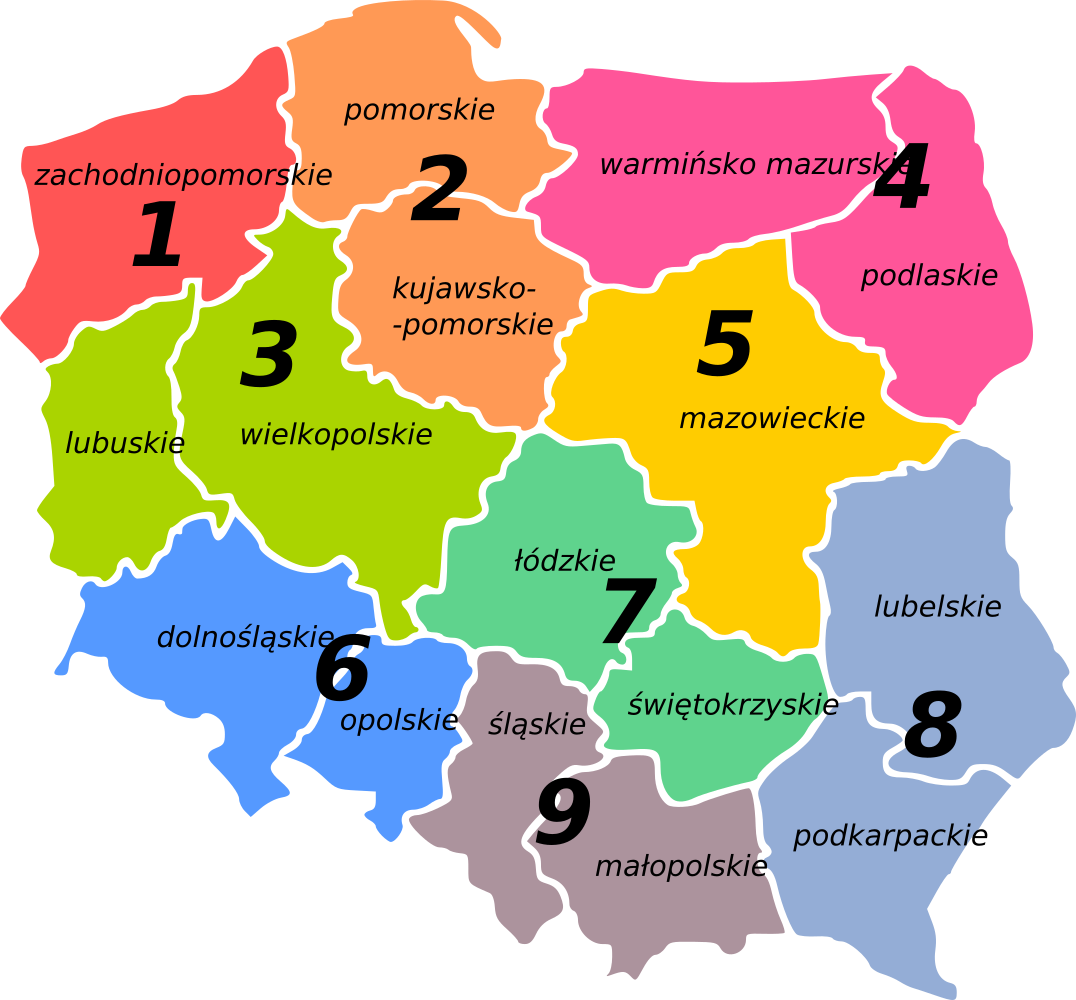
\includegraphics{Polish_HAM_Radio_Regions}
\caption{Polskie okręgi wywoławcze}
\end{figure}
\end{document}